%%
%% LaTeX template for CLEO(R)/EQEC 2019 conference papers.
%% See http://www.cleoeurope.org/submission for submission guidelines.
%%
%% Copyright (C) 2018 by Michael Riesch <michael.riesch@tum.de>
%%
%% This file may be distributed and/or modified under the conditions of
%% the LaTeX Project Public License, either version 1.2 of this license
%% or (at your option) any later version.  The latest version of this
%% license is in:
%%
%%    http://www.latex-project.org/lppl.txt
%%
%% and version 1.2 or later is part of all distributions of LaTeX version
%% 1999/12/01 or later.
%%
\documentclass{epsconf}

\title{CLEO\textsuperscript{\textregistered}/Europe-EQEC 2019, One Page
  Summary Template\\
  (Title should be centred 14 pt bold type, with Title Case\\
  Formatting - Elements, and Acronyms Should\\
  Be Capitalized)}

\author{Patrick Brown\authormark{1}, Oliver Miller\authormark{1},
  Alina Binari\authormark{2}}

\affil[1]{University of Paris Sud, 15 rue Cl\'emenceau, F-91400 Orsay, France}
\affil[2]{Universit\`a Politecnica delle Marche, IT-60131 Ancona, Italy}

\begin{document}

\maketitle

This is a sample document format for the one page extended abstract for submissions to \textbf{CLEO\textsuperscript{\textregistered}/Europe-EQEC 2019}. Although this document is provided in Microsoft Word format, the paper to be uploaded must be in \textbf{PDF format}. \textbf{Paper size should be A4 format} (210 mm x 297 mm). \textbf{Margins should be set for a 2.5 cm top, bottom, left, and right}. \textbf{For text fonts: use only 10pt Times} (roman, \textbf{bold} or \textit{italic}), and Symbol. Sans Serif Fonts such as Arial can be used in Figures. Include all equations, drawings, figures and references within the \textbf{one page limit}. Avoid asterisks, acknowledgements, job descriptions or footnotes. \textbf{Do not add page numbers}.

Please be concise in your presentation, highlighting what is novel and original about your submission. \textbf{Do not repeat the separate 35 word abstract}. Simple equations should be included in-line wherever possible, whereas more complex expressions should be centred and numbered if there are several. Figures should be relevant to the submission and preferably centred as shown below. They should be placed as close as possible to where they are mentioned in the text. Placing subfigures side-by-side is a convenient way to include multiple results within the one page limit. The figures can be provided in greyscale or colours. Figure captions should be centred beneath figures and in an 8-point font. Figure captions should be indented 1 cm on both sides and justified on both right and left sides.

\begin{figure}[h!]
  \centering
  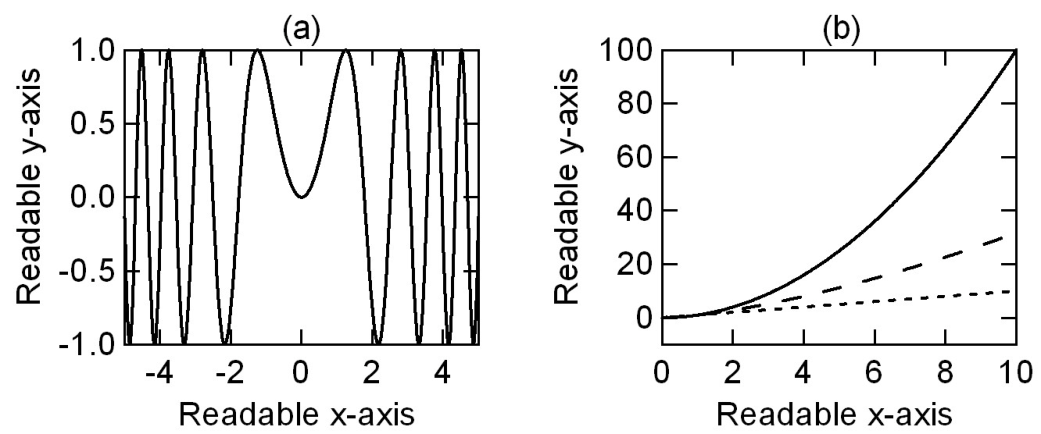
\includegraphics[width=0.9\textwidth]{sample.pdf}
  \caption{The abbreviation ``Fig.'' (for figure) should appear first,
    followed by the figure number, a	period,	and then the figure caption.}
\end{figure}

References should appear at the end of the article in the order in which they are referenced in the body of the paper. The font should be 8 point, and the references should be aligned left. A suggested format for references is given below. Within the main text, references should be designated by a number in brackets~\cite{itatani2005controlling}, and they should precede a comma or period~\cite{agrawal2001nonlinear}. Two references cited at once should be included together~\cite{itatani2005controlling, agrawal2001nonlinear}, separated by a comma, while three or more consecutive references should be indicated by the bounding numbers and a dash~\cite{itatani2005controlling, agrawal2001nonlinear, kienberger2004subfemto}.

\begin{thebibliography}{1}
  \newcommand{\enquote}[1]{``#1''}

\bibitem{itatani2005controlling}
  J.~Itatani, D.~Zeidler, J.~Levesque, D.~Villeneuve, M.~Spanner, and
  P.~Corkum,
  \enquote{Controlling high harmonic generation with molecular wave packets,}
  Phys. Rev. Lett. \textbf{94}, 123902 (2005).
  For journal articles, authors are listed first, followed by the article's
  full title in quotes, the journal's title abbreviation, the volume number
  in bold, page number, and the year in parentheses.

\bibitem{agrawal2001nonlinear}
  G.~P. Agrawal, \emph{Nonlinear Fiber Optics} (Academic Press, Boston, 2001),
  3rd ed.
  For citation of a book as a whole: authors, followed by title in italics,
  and publisher, city, and year in parenthesis.

\bibitem{kienberger2004subfemto}
  P.~Kienberger and F.~Krausz, in \enquote{Few-Cycle Laser Pulse Generation and
    Its Applications,}  F.~X. Kärtner, ed. (Springer Verlag, Berlin, 2004).
  For citation of a book chapter, authors are listed first, followed by book
  title in italics, editors, and publisher, city, and year in parenthesis.
  Chapter number may be added if applicable.

\end{thebibliography}

\end{document}
